\documentclass[11pt, a4paper, german]{article}
%\usepackage[top=2cm, bottom=2cm]{geometry}
\pagestyle{plain}

\usepackage[german]{babel}
\usepackage{amsmath}
\usepackage{amsthm}
\usepackage{amssymb}
\usepackage{graphicx}
\usepackage{tikz}
\usepackage[utf8]{inputenc}
\usepackage{caption}
\usepackage{subcaption}
\usepackage[colorlinks=true, pdfborder={0 0 0}, linkcolor=blue, citecolor=blue]{hyperref}

\newcommand{\HRule}{\rule{\linewidth}{0.5mm}}
\setlength{\parindent}{0cm}

\begin{document}
\begin{titlepage}

\begin{center}


% Oberer Teil der Titelseite:

\textsc{\LARGE Projektgruppe Angewandte Softwaretechnologie}\\[1.5cm]

\textsc{\Large Sommersemester 2015}\\[0.5cm]

\HRule \\[0.4cm] { \huge \bfseries DLVC Taverne}\\[0.2cm]
{\large \bfseries Ein Handbuch}\\[0.4cm]

\HRule \\[1.5cm]

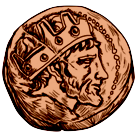
\includegraphics[width=0.6\textwidth]{./Logo3_1.png}\\[1cm]

\begin{minipage}{0.4\textwidth} \begin{flushleft} \large \emph{Author:}\\ Projektgruppe DLVC Taverne \end{flushleft} \end{minipage} \hfill \begin{minipage}{0.4\textwidth} \begin{flushright} \large \emph{Supervisor:} \\ Günther Kniesel \end{flushright} \end{minipage}

\vfill

{\large \today}

\end{center}

\end{titlepage}
\clearpage

\tableofcontents
\pagebreak

\section{Allgemeine Informationen}
\subsection{Hinweis}
Dieses Handbuch geht davon aus, dass dem Leser die Regeln von 'Die Legenden von Cystaron' (DLVC) bekannt sind. 
\subsection{Arbeitsgruppe}
Das Programm 'DLVC Taverne' ist 2015 im Rahmen der Projektgruppe 'Angewandte Softwaretechnologie' unter der Leitung von Dr. Kniesel entstanden. Die Entwickler waren:
\begin{itemize}
	\item[] Britta Heymann
	\item[] Andreas Kofer
	\item[] Nooshin Naghavi
	\item[] Boris Prochnau
\end{itemize}

\newpage
\section{Das Hauptmenü}
Das Hauptmenü besteht aus zwei vertikal getrennten Bereichen, den Buttons für die Hauptfunktionen und der Gruppenauswahl (siehe Abb. \ref{fig:Hauptmenue1}). Außerdem findet sich (wie auf fast jedem Fenster) ein Hilfe Button am rechten unteren, welches über das aktuelle Fenster informieren kann.\\
\begin{figure}
\centering
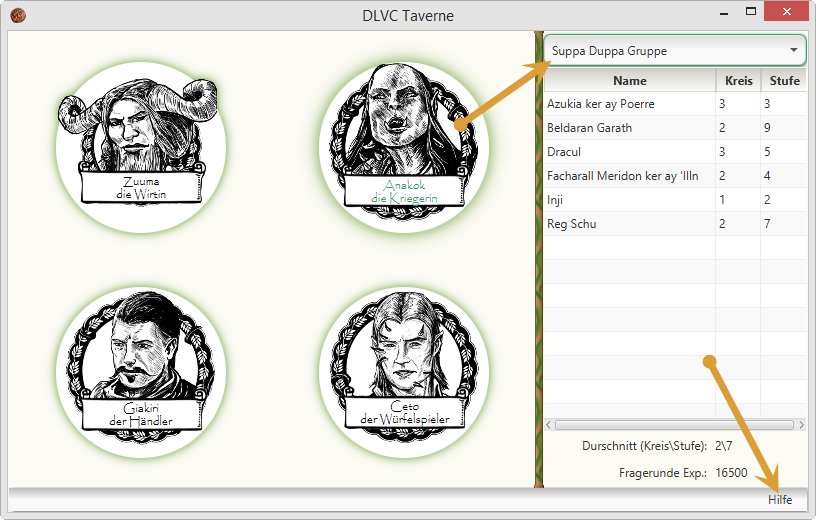
\includegraphics[width=1\linewidth]{Bilder/Hauptmenue1}
\caption{Hauptmenü}
\label{fig:Hauptmenue1}
\end{figure}


\subsection{Button Bereich}
%\textbf{Button Bereich:}\\
Im linken Bereich finden sich vier Buttons um auf die Grundfunktionen des Programm zuzugreifen.
\begin{itemize}
	\item[] \textbf{Charaktermanager}: Hier können Spielercharaktere und Nichtspieler-Charakter-Typen angelegt, sowie Abenteuergruppen verwaltet werden.
	\item[] \textbf{Kampf}: Das führt zu einer Teilnehmerauswahl für die Teilnehmer des Kampfes (Spieler und Gegner). Anschließend kann ein Kampfhelfer für den Kampf gestartet werden.
	\item[] \textbf{Händler}: Hier können alle Gegenstände und Ausrüstungsteile erstellt, gesucht und anderweitig verwaltet werden.
	\item[] \textbf{Würfeln}: Hier können diverse Würfelwürfe simuliert werden.
\end{itemize}

\subsection{Gruppenauswahl}
Im rechten Bereich findet sich die Gruppenauswahl. Jede zuvor im Charaktermanger zusammengestellte Gruppe kann in Combo-Box ganz oben ausgewählt werden, woraufhin alle Mitglieder mit Kreis und Level angezeigt werden.

\newpage

\section{Der Charaktermanager}
\subsection{Der Gruppenmanager}
\subsection{Der Charaktermanager}
\subsection{Der Gegnermanager}

\section{Der Kampf}
\subsection{Die Gegnerrunde}
\subsection{Die Spielerrunde}
\subsection{Das Kampfende}

\section{Der Händler}
\subsection{Allgemein}
\subsection{Inventar}
\subsection{Rüstung und Waffen}

\section{Würfeln}


\end{document}